\documentclass[usenames,dvipsnames]{beamer}


%\usepackage[utf8]{inputenc}
\usepackage{hyperref}
\usepackage{wasysym}
\usepackage{siunitx}
\usepackage{graphicx}


%\usepackage{xurl}
%\usepackage{cite}
\usepackage{framed}
%\usepackage{breqn}
\usepackage{amsfonts}
\usepackage{amsmath}
\usepackage{xcolor}
\usepackage{multicol}
%\usepackage{natbib}
%\usepackage[style=verbose]{biblatex}


\usetheme{Warsaw}
%\usecolortheme{crane}
%\usecolortheme{seahorse}
%\usecolortheme{beaver}
%\definecolor{UBCblue}{rgb}{0.04706, 0.13725, 0.26667} % UBC Blue (primary)
\definecolor{UBCblue}{rgb}{0.0, 0.134, 0.413} % UBC Blue (primary)
\usecolortheme[named=UBCblue]{structure}
%\usecolortheme[named=Mahogany]{structure}



\setbeamertemplate{navigation symbols}{}
\setbeamertemplate{headline}{}
%\renewcommand{\insertnavigation}[1]{}
%\def\insertnavigation#1{\relax}
%\usepackage[hyphens]{url}
%\pdfpkresolution=150
%\pdfpkmode={supre}



\usepackage[style=ieee]{biblatex}
\bibliography{kovzol,external}

\newtheorem{conjecture}{Conjecture}
\newcommand{\Exists}[1]{\underset{#1}{\exists}\,}


\expandafter\def\expandafter\insertshorttitle\expandafter{%
  \insertshorttitle\hfill%
  \hfill
  \textcolor{Mahogany!20}{\insertframenumber/\inserttotalframenumber}}


\tolerance10000

%\bibliographystyle{splncs}
% \includegraphics[width=0.4\textwidth]{watt}


\title[Faithful real-time animation via CAD]{%
Faithful real-time animation of \\ parametrized (semi-)algebraic expressions
\\ via cylindrical algebraic decomposition}

\author[Brown, Kov\'acs and Recio]{
Christopher W.~Brown \inst{1} \and
Zolt\'an Kov\'acs \inst{2} \and
Tomás Recio \inst{3}
\\
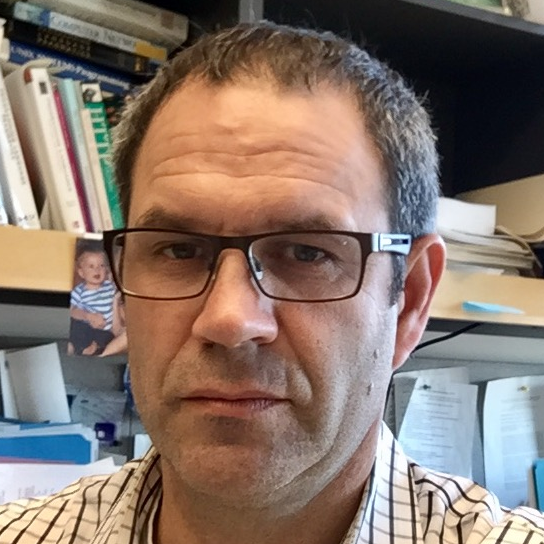
\includegraphics[width=0.8cm]{brown544}
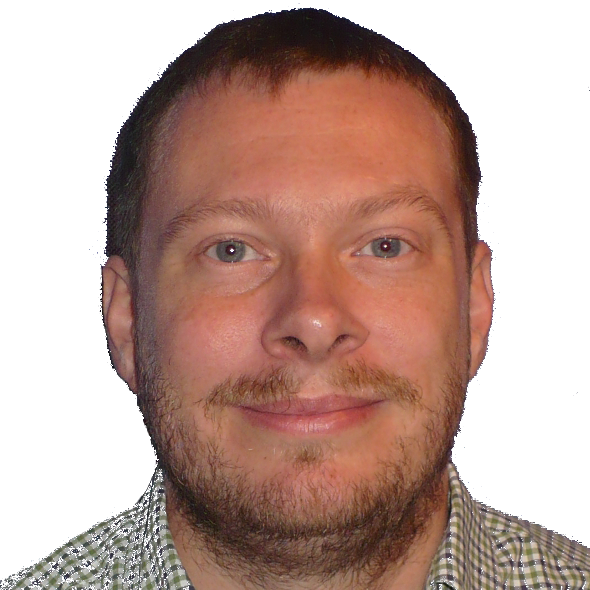
\includegraphics[width=0.8cm]{kovacs590}

\includegraphics[width=0.8cm]{tomas96}
}
\institute{
\inst{1} United States Naval Academy, Annapolis, MD, USA \and %
\inst{2} The Private University College of Education of the Diocese of Linz, Austria \and %
\inst{3} Nebrija University, Madrid, Spain}
\date{ISSAC 2023, July 2023\\
{\vskip0.3cm \tiny ${}^{23}$ Authors are supported by the grant
PID2020-113192GB-I00 from the Spanish MICINN.
}
}


\begin{document}
\maketitle              % typeset the title of the contribution



\begin{frame}
\frametitle{Abstract}

We present some current improvements, implemented in the software package \textit{GeoGebra Discovery},
that combine symbolic computation and graphics algorithms to faithfully visualize (semi-)algebraic expressions.
Our implementation allows fluid animation of set of (semi-)algebraic sets of dimension 1 in
a desktop application or a web browser. We use the \textsc{Tarski} library to create a cylindrical algebraic
decomposition of the input, and its \texttt{plot2d} command, which is processed further in GeoGebra Discovery,
to provide the user with a familiar look and feel.
\end{frame}

\begin{frame}
\frametitle{Message}

Outreach$\ldots$
\begin{itemize}
\item potentially 100,000,000 of young learners and students with
\item fast state-of-the-art symbolic computation
\item on all popular native platforms (Windows, Mac, Linux) and the web.
\end{itemize}

\end{frame}




\begin{frame}
\frametitle{GeoGebra: open platform for teaching and learning math}
\framesubtitle{\href{https://www.geogebra.org}{geogebra.org}}
\begin{center}

\includegraphics[width=1\textwidth]{www-geogebra-org} \\
\end{center}
\end{frame}

\begin{frame}
\frametitle{GeoGebra Discovery: an experimental version of GeoGebra}
\framesubtitle{\href{https://github.com/kovzol/geogebra-discovery}{github.com/kovzol/geogebra-discovery}}
\begin{center}
\includegraphics<1>[width=0.9\textwidth]{g1}%
\includegraphics<2>[width=0.9\textwidth]{g2}%
\includegraphics<3>[width=0.9\textwidth]{g2b}
\end{center}
\end{frame}

\begin{frame}
\frametitle{Software releases at Snapcraft (May 2023)}
\framesubtitle{Linux installations only (snap packages)}
\begin{center}
\includegraphics<1>[width=1\textwidth]{territories}%
\includegraphics<2>[width=1\textwidth]{gg-snap}
\end{center}
\end{frame}



\begin{frame}
\frametitle{\textsc{Tarski}: A free C++ library$\ldots$}
\framesubtitle{$\ldots$for manipulating connectives of (semi-)algebraic expressions}
\begin{center}
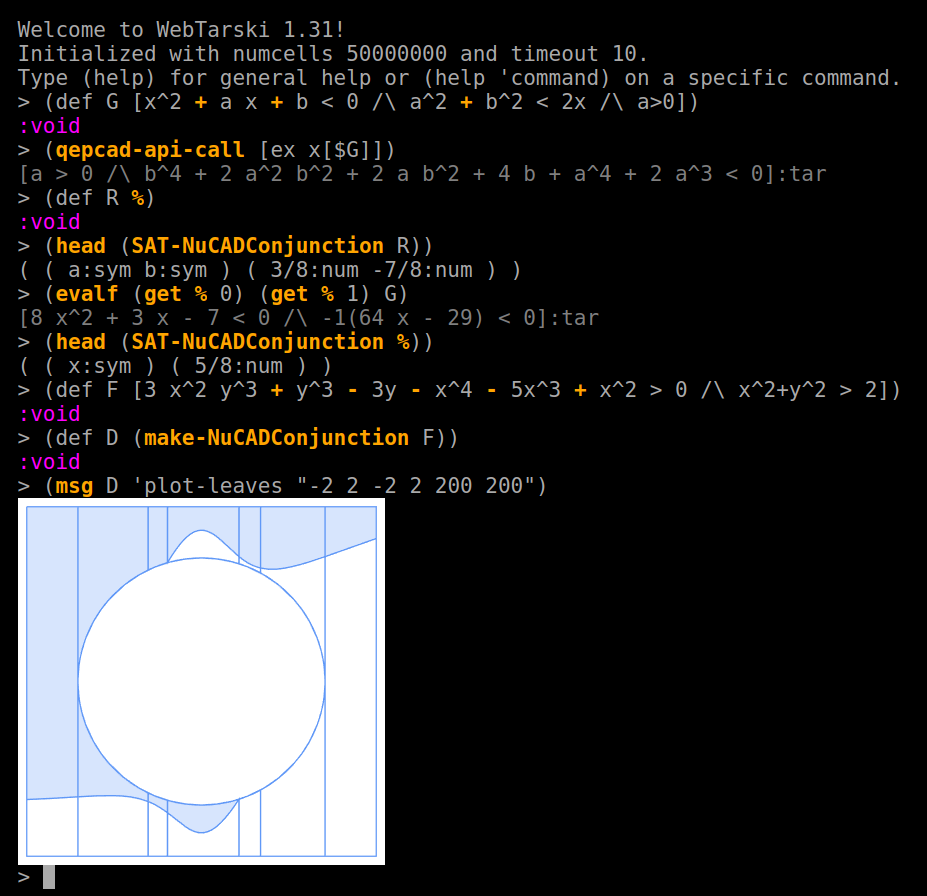
\includegraphics[width=0.7\textwidth]{webtarski}
\end{center}
\end{frame}

\begin{frame}
\frametitle{The \texttt{Plot2D} command in GeoGebra Discovery}
\framesubtitle{It communicates with the \texttt{plot2d} command in \textsc{Tarski}}
GeoGebra Discovery input: logical connective(s) of (semi-)algebraic expression(s). \pause
It is forwarded to an embedded version of \textsc{Tarski}. \textsc{Tarski}'s \texttt{plot2d}
command creates an SVG output which is plotted by GeoGebra Discovery. \pause

Examples:
\begin{itemize}
\item \texttt{Plot2D($x^2+y^2=x^3$)} \pause
\item \texttt{Plot2D($x^2+y^2\leq x^3$)} \pause
\item After creating a slider $a$ and then \texttt{Plot2D($x^2+y^2\leq a x^3-xy^4+1$)}:
\url{https://autgeo.online/index.html?command=Slider(-2,5);x\%5E2--y\%5E2\%3C=a*x\%5E3-x\%20y\%5E4--1;StartAnimation(a,true)}
\item An implicit curve that was created by GeoGebra's geometric construction steps dynamically (via Gröbner bases)
can be re-plotted accurately.
\end{itemize}
\end{frame}

\begin{frame}
\frametitle{Re-plotting an implicit algebraic curve accurately}
\framesubtitle{Speed allows real-time animation of the coupler curves (degree 6) of 4-bar linkages}
\begin{center}
\includegraphics<1>[width=0.7\textwidth]{Chebyshev-fps1bc}%
\includegraphics<2>[width=0.7\textwidth]{chebyshev6b}
\end{center}
\end{frame}



\end{document}
